\documentclass[11pt]{article}

\usepackage[margin=1in]{geometry}
\usepackage[T1]{fontenc}
\usepackage{lmodern}
\usepackage{microtype}
\usepackage{amsmath,amssymb,amsthm,mathtools}
\usepackage{mathrsfs}
\usepackage[dvipsnames]{xcolor}
\usepackage[most]{tcolorbox}
\usepackage{tikz}
\usetikzlibrary{decorations.markings,patterns}
\usepackage{enumitem}
\usepackage{tocloft}
\usepackage[hidelinks]{hyperref}

\definecolor{courseblue}{HTML}{1F4E79}
\definecolor{lightblue}{HTML}{EAF2F8}
\definecolor{lightgreen}{HTML}{EAF7EA}
\definecolor{lightpink}{HTML}{FCE8EF}
\definecolor{lightyellow}{HTML}{FFF8D6}
\definecolor{warningyellow}{HTML}{D6A000}
\definecolor{exercisebg}{HTML}{FDEAEA}
\definecolor{exerciseframe}{HTML}{B54040}
\definecolor{examplebg}{HTML}{F4FAFE}
\definecolor{exampleframe}{HTML}{85C1E9}
\definecolor{darkgray}{HTML}{333333}
\definecolor{lightorange}{HTML}{FDEBD8}
\definecolor{orangeframe}{HTML}{E08A3C}
\definecolor{remarkbg}{HTML}{F3EEFB}
\definecolor{remarkframe}{HTML}{9B7FC9}

\setlength{\parindent}{0pt}
\setlength{\parskip}{0.45em}
\setlist[itemize]{topsep=0.25em,itemsep=0.15em}
\renewcommand{\cftsecleader}{\cftdotfill{\cftdotsep}}
\renewcommand{\cftsubsecleader}{\cftdotfill{\cftdotsep}}

\theoremstyle{plain}
\newtheorem{theorem}{Theorem}[section]
\newtheorem{proposition}[theorem]{Proposition}
\newtheorem{lemma}[theorem]{Lemma}
\newtheorem{corollary}[theorem]{Corollary}
\theoremstyle{definition}
\newtheorem{definition}[theorem]{Definition}
\newtheorem{example}[theorem]{Example}
\newtheorem{exercise}[theorem]{Exercise}
\newtheoremstyle{boldremark}
  {3pt}{3pt}{\normalfont}{}{\bfseries}{.}{.5em}
  {\thmname{#1}\thmnumber{ #2}\thmnote{ (#3)}}
\theoremstyle{boldremark}
\newtheorem*{remark}{Remark}
\theoremstyle{remark}
\newtheorem*{fact}{Fact}
\newtheorem*{warning}{Warning}

\tcolorboxenvironment{definition}{
  enhanced,
  unbreakable,
  colback=lightgreen,
  colframe=ForestGreen,
  boxrule=0.7pt,
  arc=2pt,
  left=6pt,
  right=6pt,
  top=5pt,
  bottom=5pt
}

\tcolorboxenvironment{remark}{
  enhanced,
  colback=remarkbg,
  colframe=remarkframe,
  before upper={\setlength{\parskip}{0.5em}},
  boxrule=0.7pt,
  arc=2pt,
  left=6pt,
  right=6pt,
  top=5pt,
  bottom=5pt
}

\tcolorboxenvironment{warning}{
  enhanced,
  colback=lightyellow,
  colframe=warningyellow,
  boxrule=0.7pt,
  arc=2pt,
  left=6pt,
  right=6pt,
  top=5pt,
  bottom=5pt
}

\tcolorboxenvironment{exercise}{
  enhanced,
  colback=exercisebg,
  colframe=exerciseframe,
  boxrule=1pt,
  arc=2pt,
  left=6pt,
  right=6pt,
  top=5pt,
  bottom=5pt
}

\tcolorboxenvironment{example}{
  enhanced,
  colback=examplebg,
  colframe=exampleframe,
  boxrule=0.7pt,
  arc=2pt,
  left=6pt,
  right=6pt,
  top=5pt,
  bottom=5pt
}

\numberwithin{equation}{section}

\newcommand{\C}{\mathbb{C}}
\newcommand{\R}{\mathbb{R}}
\newcommand{\N}{\mathbb{N}}
\newcommand{\Z}{\mathbb{Z}}
\DeclareMathOperator{\Log}{Log}
\DeclareMathOperator{\Arg}{Arg}

\DeclareMathOperator{\Hol}{\mathcal{H}\mathrm{ol}}
\DeclareMathOperator{\Real}{Re}
\DeclareMathOperator{\Imag}{Im}
\newcommand{\A}{\mathcal{A}}
\newcommand{\CT}{\C[[T]]}
\newcommand{\CLT}{\C((T))}
\tcbset{breakable}
% Compact spacing around diagrams; keep the main text at 11pt.
\newenvironment{lecturefigure}
 {\par\addvspace{0.25em}\begingroup\setlength{\parskip}{0pt}\centering}
 {\par\endgroup\addvspace{0.25em}}
\begin{document}

\begin{center}
  \colorbox{lightblue}{%
    \begin{minipage}{0.94\textwidth}
      \vspace{0.55em}
      \begin{tabular*}{\textwidth}{@{\extracolsep{\fill}}lr}
        {\color{courseblue}\bfseries\LARGE Lecture 28} &
        {\color{courseblue}\bfseries\LARGE MATH 411}\\[0.35em]
        \textbf{Fall 2026} & \textbf{Date: Nov 23, 2026}\\
        & \textbf{Instructor: Manish Patnaik}
      \end{tabular*}
      \vspace{0.45em}
    \end{minipage}}
\end{center}

\setcounter{tocdepth}{1}
\tableofcontents
\vspace{0.45em}

% Handwritten Lecture 26, Nov. 21, pp. 1--3.
\section{Schwarz's lemma}
Given open sets $U$ and $V$, we can ask whether there is an analytic
isomorphism $U\to V$. When $V=U$, we can ask for \emph{all} such maps.
An analytic isomorphism from $U$ to itself is called an
\emph{automorphism} of $U$. We will determine the automorphisms of the
unit disc $D=\{z\in\C:|z|<1\}$, beginning with maps that fix the origin.

\begin{lemma}[Schwarz's lemma]\label{lem:schwarz}
Let $f:D\to D$ be holomorphic with $f(0)=0$. Then
\begin{equation}
 |f(z)|\leq |z|\quad(z\in D),\qquad |f'(0)|\leq 1.
\end{equation}
If $|f(z_0)|=|z_0|$ for some $z_0\in D\setminus\{0\}$, or if
$|f'(0)|=1$, then $f$ is a rotation: there is a $\varphi\in\R$ such
that $f(z)=e^{i\varphi}z$ for every $z\in D$.
\end{lemma}
\begin{proof}
Since $f(0)=0$, its Taylor series starts with
$f(z)=a_1z+a_2z^2+\cdots$. Thus $g(z)=f(z)/z$ extends holomorphically
across $0$ by taking $g(0)=a_1=f'(0)$.

Fix $0<r<1$ and let $D_r=\{z:|z|<r\}$. On the circle $|z|=r$ we have
\begin{equation}\label{g:bd}
 |g(z)|=\frac{|f(z)|}{r}\leq\frac{1}{r}.
\end{equation}
Since $\overline{D_r}\subset D$, the maximum modulus principle gives
the same bound throughout $D_r$.
\begin{lecturefigure}
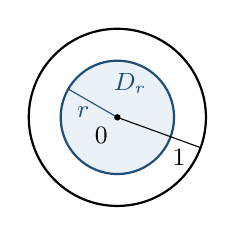
\begin{tikzpicture}[>=stealth,scale=0.9,font=\small]
 \draw[thick] (0,0) circle (1.25);
 \filldraw[fill=lightblue,draw=courseblue,thick] (0,0) circle (0.80);
 \draw[courseblue] (0,0) -- (150:0.80) node[midway,below left,inner sep=1pt] {$r$};
 \draw (0,0) -- (-20:1.25) node[pos=0.74,below] {$1$};
 \fill (0,0) circle (1.3pt) node[below left] {$0$};
 \node[courseblue] at (0.18,0.48) {$D_r$};
\end{tikzpicture}

{\small The bound on $|z|=r$ controls $g$ on the shaded disc.}
\end{lecturefigure}
For a fixed $z\in D$, we may choose any $r$ with $|z|<r<1$.
Then $|g(z)|\leq 1/r$ for every such $r$, and letting $r$ tend to $1$ gives $|g(z)|\leq1$.
Hence $|f(z)|\leq|z|$, and evaluating at $0$ gives $|f'(0)|=|g(0)|\leq1$.

If $|f(z_0)|=|z_0|$ at a nonzero $z_0$, then $|g(z_0)|=1$.
If $|f'(0)|=1$, then $|g(0)|=1$. In either case $|g|$ attains its
maximum inside $D$. By the maximum modulus principle, $g$ is a
constant of modulus $1$, say $e^{i\varphi}$. Thus $f(z)=e^{i\varphi}z$.
\end{proof}

% Handwritten Lecture 26, pp. 4--7.
\section{Automorphisms of the unit disc}
Write $\operatorname{Aut}(D)$ for the group of analytic automorphisms
of $D$ under composition. The rotations $r_\varphi(z)=e^{i\varphi}z$
belong to this group, with inverse $r_{-\varphi}$. To move the origin
to another point of $D$, we use the following maps.

\begin{proposition}[Blaschke factors]\label{prop:disc-involution}
For each $\alpha\in D$, the map
\begin{equation}
 \psi_\alpha(z)=\frac{\alpha-z}{1-\overline\alpha z}
\end{equation}
is an automorphism of $D$ that interchanges $0$ and $\alpha$ and is its
own inverse.
\end{proposition}

\begin{proof}
The denominator is nonzero on $\overline D$ since
$|\overline\alpha z|\leq|\alpha|<1$ there. Thus $\psi_\alpha$ is
holomorphic on a neighborhood of $\overline D$. Substitution gives
$\psi_\alpha(0)=\alpha$ and $\psi_\alpha(\alpha)=0$.

On $|z|=1$, the identity $1-\overline\alpha z=z\,\overline{(z-\alpha)}$
gives $|1-\overline\alpha z|=|z-\alpha|$. Hence $|\psi_\alpha|=1$
on the boundary. The map is nonconstant (for $\alpha=0$ it is $-z$,
and otherwise it interchanges two distinct points). The maximum modulus
principle now gives $|\psi_\alpha(z)|<1$ throughout $D$.

It remains to check the inverse. For $z\in D$, clearing the common
denominator $1-\overline\alpha z$ gives
\begin{equation}
 \psi_\alpha(\psi_\alpha(z))
 =\frac{\alpha(1-\overline\alpha z)-(\alpha-z)}
        {(1-\overline\alpha z)-\overline\alpha(\alpha-z)}
 =\frac{(1-|\alpha|^2)z}{1-|\alpha|^2}=z.
\end{equation}
Thus $\psi_\alpha:D\to D$ is bijective with holomorphic inverse
$\psi_\alpha$.
\end{proof}

\begin{remark}
	These maps appeared in Homework~1, Problem~4, with $w$ in place of
	$\alpha$. In part~(b), computing $F\circ F$ was the hint for proving
	bijectivity.
\end{remark}

\begin{theorem}[Automorphisms of the unit disc]\label{thm:disc-automorphisms}
Every $f\in\operatorname{Aut}(D)$ has the form
\begin{equation}
 \boxed{\displaystyle f(z)=e^{i\varphi}
       \frac{\alpha-z}{1-\overline\alpha z}}
 \qquad (\alpha\in D,\ \varphi\in\R).
\end{equation}
Conversely, every map of this form is an automorphism of $D$.
\end{theorem}
\begin{proof}
Choose $\alpha=f^{-1}(0)$. The automorphism $g=f\circ\psi_\alpha$
fixes $0$, since $g(0)=f(\alpha)=0$. Its inverse fixes $0$ as well.
Applying Schwarz's lemma to $g$ at $z$ and to $g^{-1}$ at $g(z)$ gives
\begin{equation}
 |g(z)|\leq|z|=|g^{-1}(g(z))|\leq |g(z)|.
\end{equation}
Hence $|g(z)|=|z|$ throughout $D$. By the equality case of Schwarz's
lemma, $g=r_\varphi$ for some $\varphi\in\R$. Composing on the right
with $\psi_\alpha$ gives $f=r_\varphi\circ\psi_\alpha$. Conversely,
this composition is an automorphism because both factors are.
\end{proof}

\begin{corollary}\label{cor:disc-rotation}
An automorphism of $D$ that fixes $0$ is a rotation.
\end{corollary}

\newpage
\begin{remark}[Transporting automorphisms]
The Riemann mapping theorem gives an analytic isomorphism $h:U\to D$
for every nonempty simply connected domain $U\subsetneq\C$. Once such
an $h$ is chosen, each automorphism $A$ of $D$ gives an automorphism
$h^{-1}\circ A\circ h$ of $U$. Every automorphism $B$ of $U$ arises
in this way by taking $A=h\circ B\circ h^{-1}$.
\begin{lecturefigure}
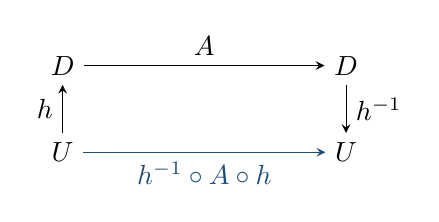
\begin{tikzpicture}[>=stealth,baseline=(current bounding box.center)]
 \node (d1) at (0,1.1) {$D$}; \node (d2) at (3.6,1.1) {$D$};
 \node (u1) at (0,0) {$U$};    \node (u2) at (3.6,0) {$U$};
 \draw[->] (u1) -- node[left] {$h$} (d1);
 \draw[->] (d1) -- node[above] {$A$} (d2);
 \draw[->] (d2) -- node[right] {$h^{-1}$} (u2);
 \draw[->,courseblue] (u1) -- node[below] {$h^{-1}\circ A\circ h$} (u2);
\end{tikzpicture}
\end{lecturefigure}
\end{remark}

% Source: handwritten Lecture 27, Nov. 23, pp. 1--8.
\section{The upper half-plane and the unit disc}

Write $\mathbb H=\{z\in\C:\Imag z>0\}$ for the upper half-plane.
The classification of $\operatorname{Aut}(D)$ in
Theorem~\ref{thm:disc-automorphisms} gives a classification of
$\operatorname{Aut}(\mathbb H)$ once we have an analytic isomorphism
between $\mathbb H$ and $D$.

\begin{proposition}[The Cayley map]\label{prop:cayley}
The maps
\begin{equation}
 F(z)=\frac{i-z}{i+z},\qquad G(w)=i\frac{1-w}{1+w}
\end{equation}
are inverse analytic isomorphisms between $\mathbb H$ and $D$.
\end{proposition}
\begin{proof}
The only pole of $F$ is at $-i$, so $F$ is holomorphic on $\mathbb H$.
For $z=x+iy$ with $y>0$,
\begin{equation}
 |F(z)|^2=\frac{x^2+(1-y)^2}{x^2+(1+y)^2}<1.
\end{equation}
For $w\in D$, $1+w\ne0$, so $G$ is holomorphic on $D$, and
$\Imag G(w)=\Real\bigl((1-w)/(1+w)\bigr)=(1-|w|^2)/|1+w|^2>0$.
Solving $w=F(z)$ gives $z=G(w)$, so these maps are inverses.
In particular, $F(i)=0$ and $G(0)=i$.
\end{proof}

\begin{lecturefigure}
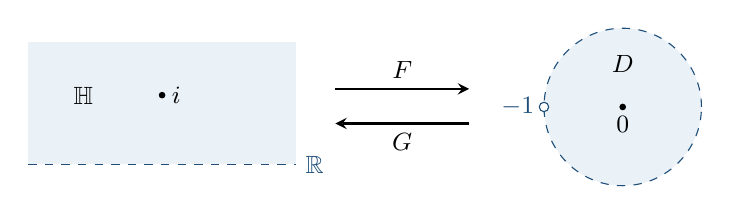
\begin{tikzpicture}[>=stealth,font=\small]
 \fill[lightblue] (-1.7,0) rectangle (1.7,1.55);
 \draw[courseblue,dashed] (-1.7,0) -- (1.7,0) node[right] {$\R$};
 \fill (0,0.88) circle (1.2pt) node[right] {$i$};
 \node at (-1,0.87) {$\mathbb H$};
 \draw[->,thick] (2.2,0.96) -- node[above] {$F$} (3.9,0.96);
 \draw[<-,thick] (2.2,0.52) -- node[below] {$G$} (3.9,0.52);
 \filldraw[fill=lightblue,draw=courseblue,dashed] (5.85,0.73) circle (1);
 \fill (5.85,0.73) circle (1.2pt) node[below] {$0$};
 \draw[courseblue,fill=white] (4.85,0.73) circle (1.7pt) node[left] {$-1$};
 \node at (5.85,1.27) {$D$};
\end{tikzpicture}
\end{lecturefigure}

\begin{exercise}[The boundary under the Cayley map]
For $x\in\R$, verify that
\begin{equation}
 F(x)=\frac{1-x^2}{1+x^2}+i\frac{2x}{1+x^2}.
\end{equation}
Show that $F(\R)=\{w:|w|=1\}\setminus\{-1\}$, and that
$F(x)\to-1$ as $|x|\to\infty$. For surjectivity on the punctured
circle, use $G$.
\end{exercise}

\section{Automorphisms of the upper half-plane}

\begin{definition}[Fractional linear transformations]
Let $\mathrm{SL}(2,\R)$ be the group of real $2\times2$ matrices of
determinant $1$. To $g=\left(\begin{smallmatrix}a&b\\c&d\end{smallmatrix}\right)$
in this group associate the \emph{fractional linear transformation}
\begin{equation}
 \phi_g(z)=\frac{az+b}{cz+d}.
\end{equation}
\end{definition}

\begin{example}[Horizontal translation]
For $x\in\R$, let
\begin{equation}
 T=\begin{pmatrix}1&x\\0&1\end{pmatrix},
 \qquad \phi_T(z)=z+x.
\end{equation}
The map shifts every point horizontally by $x$, preserving its imaginary
part. The picture shows $x>0$.

\begin{lecturefigure}
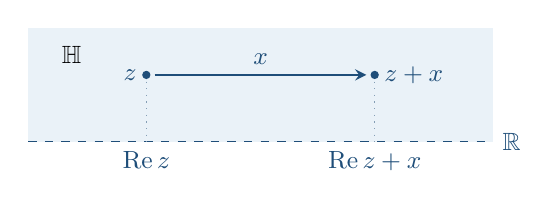
\begin{tikzpicture}[>=stealth,font=\small]
 \fill[lightblue] (-0.35,0) rectangle (5.55,1.45);
 \draw[courseblue,dashed] (-0.35,0) -- (5.55,0) node[right] {$\R$};
 \node at (0.2,1.1) {$\mathbb H$};
 \draw[courseblue!55,dotted] (1.15,0.85) -- (1.15,0) node[below,text=courseblue] {$\Real z$};
 \draw[courseblue!55,dotted] (4.05,0.85) -- (4.05,0) node[below,text=courseblue] {$\Real z+x$};
 \draw[->,courseblue,thick,shorten <=3pt,shorten >=3pt]
   (1.15,0.85) -- node[above] {$x$} (4.05,0.85);
 \fill[courseblue] (1.15,0.85) circle (1.5pt) node[left] {$z$};
 \fill[courseblue] (4.05,0.85) circle (1.5pt) node[right] {$z+x$};
\end{tikzpicture}
\end{lecturefigure}
\end{example}

\begin{example}[Inversion]
Let
\begin{equation}
 S=\begin{pmatrix}0&-1\\1&0\end{pmatrix},
 \qquad \phi_S(z)=-\frac{1}{z}.
\end{equation}
The map fixes $i$ and sends $z=re^{i\theta}$ to
$r^{-1}e^{i(\pi-\theta)}$. In the picture, $z=1+i$ maps to $(-1+i)/2$.

\begin{lecturefigure}
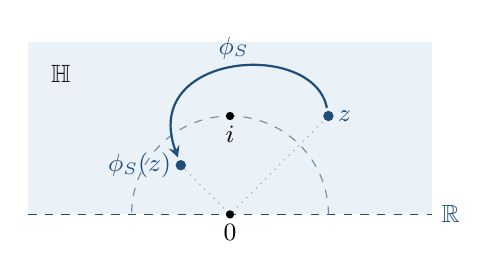
\begin{tikzpicture}[>=stealth,font=\small,scale=1.25]
 \fill[lightblue] (-2.05,0) rectangle (2.05,1.75);
 \draw[courseblue,dashed] (-2.05,0) -- (2.05,0) node[right] {$\R$};
 \node at (-1.72,1.43) {$\mathbb H$};
 \draw[courseblue!65,dashed] (1,0) arc[start angle=0,end angle=180,radius=1];
 \draw[courseblue!55,dotted] (-0.5,0.5) -- (0,0) -- (1,1);
 \draw[->,courseblue,thick,shorten <=3pt,shorten >=3pt]
   (1,1) .. controls (0.85,1.78) and (-0.92,1.65) .. node[midway,above] {$\phi_S$} (-0.5,0.5);
 \fill (0,0) circle (1.2pt) node[below] {$0$};
 \fill (0,1) circle (1.2pt) node[below] {$i$};
 \fill[courseblue] (1,1) circle (1.5pt) node[right] {$z$};
 \fill[courseblue] (-0.5,0.5) circle (1.5pt) node[left] {$\phi_S(z)$};
\end{tikzpicture}
\end{lecturefigure}

More generally, for $\lambda\in\R\setminus\{0\}$ the matrix
$\left(\begin{smallmatrix}0&\lambda\\-\lambda^{-1}&0\end{smallmatrix}\right)$
gives $z\mapsto-\lambda^2/z$.
\end{example}

Now let $g=\left(\begin{smallmatrix}a&b\\c&d\end{smallmatrix}\right)\in\mathrm{SL}(2,\R)$
and $z\in\mathbb H$. If $c\ne0$, the denominator $cz+d$ vanishes only at
the real point $-d/c$; if $c=0$, then $ad=1$ gives $d\ne0$. Multiplying
numerator and denominator by $\overline{cz+d}$ yields
\begin{equation}
 \Imag\phi_g(z)=\frac{(ad-bc)\Imag z}{|cz+d|^2}
               =\frac{\Imag z}{|cz+d|^2}.
\end{equation}
Thus $\phi_g$ is holomorphic and maps $\mathbb H$ into itself.

\newpage
\begin{exercise}[Composition]
For $g_1,g_2\in\mathrm{SL}(2,\R)$, check by substitution that
$\phi_{g_1g_2}=\phi_{g_1}\circ\phi_{g_2}$. Deduce that for
$g=\left(\begin{smallmatrix}a&b\\c&d\end{smallmatrix}\right)\in\mathrm{SL}(2,\R)$,
$\phi_{g^{-1}}$ is the inverse of $\phi_g$, where
$g^{-1}=\left(\begin{smallmatrix}d&-b\\-c&a\end{smallmatrix}\right)$.
Conclude that $\phi_g\in\operatorname{Aut}(\mathbb H)$.
\end{exercise}

\begin{theorem}[Automorphisms of $\mathbb H$]
Every analytic automorphism of $\mathbb H$ is $\phi_g$ for some
$g\in\mathrm{SL}(2,\R)$. Conversely, every such $\phi_g$ is an
analytic automorphism of $\mathbb H$.
\end{theorem}
\begin{proof}
The converse follows from the computation above and the preceding
exercise. Now let $\psi\in\operatorname{Aut}(\mathbb H)$. First
suppose $\psi(i)=i$. The disc automorphism $F\circ\psi\circ G$
fixes $0$ because $G(0)=i$ and $F(i)=0$. Corollary~\ref{cor:disc-rotation} gives
$(F\circ\psi\circ G)(w)=e^{i\theta}w$ for some $\theta\in\R$.

For $z\in\mathbb H$, substitute $w=F(z)$. Since $G(F(z))=z$, the rotation
identity becomes $F(\psi(z))=e^{i\theta}F(z)$. Applying $G$ to both sides
gives $\psi(z)=G(e^{i\theta}F(z))$.
Substituting the formulas for $F$ and $G$ and clearing the fractions gives
\begin{equation}\label{eq:conjugated-rotation}
 \psi(z)
   =i\frac{(i+z)-e^{i\theta}(i-z)}{(i+z)+e^{i\theta}(i-z)}
   =i\frac{i(1-e^{i\theta})+z(1+e^{i\theta})}
           {i(1+e^{i\theta})+z(1-e^{i\theta})}.
\end{equation}
Absorb the leading $i$ into the numerator of \eqref{eq:conjugated-rotation}
and read off the coefficients of $z$ and the constant terms. Then
\begin{equation}
 \psi(z)=\frac{az+b}{cz+d},
 \qquad
 M=\begin{pmatrix}a&b\\c&d\end{pmatrix}
   =\begin{pmatrix}
      i(1+e^{i\theta}) & e^{i\theta}-1\\
      1-e^{i\theta} & i(1+e^{i\theta})
    \end{pmatrix}.
\end{equation}
Scaling all four coefficients by the same nonzero factor leaves
$\psi$ unchanged. Put $u=\theta/2$. Using $1+e^{i\theta}=2e^{iu}\cos u$
and $1-e^{i\theta}=-2ie^{iu}\sin u$, we obtain the real matrix
\begin{equation}
 k=\frac{1}{2ie^{iu}}M
   =\begin{pmatrix}\cos u&\sin u\\-\sin u&\cos u\end{pmatrix}.
\end{equation}
Thus $\psi=\phi_k$, and $\det k=\cos^2 u+\sin^2 u=1$.

Now let $\psi(i)=w=x+iy\in\mathbb H$. The map $z\mapsto(z-x)/y$
takes $w$ to $i$ and is $\phi_h$ for
\begin{equation}
 h=\begin{pmatrix}1/\sqrt y&-x/\sqrt y\\0&\sqrt y\end{pmatrix}.
\end{equation}
Then $\phi_h\circ\psi$ fixes $i$ and hence equals some $\phi_k$
from the first part. Thus $\psi=\phi_{h^{-1}k}$.
\end{proof}

\end{document}
